\section{Lernfeld 2: Arbeitsplätze nach Kundenwunsch ausstatten}

\begin{figure}
    [H]
    \centering
    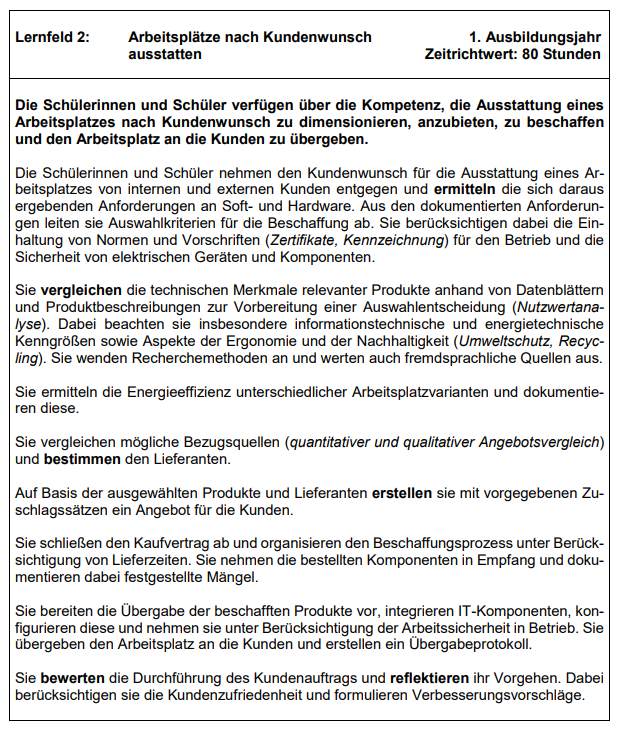
\includegraphics[width=\textwidth]{figures/lernfeld2.png}
    \caption{Lernfeld 2}
    \label{fig:lernfeld2}
\end{figure}

\subsection{Nutzwertanalyse}
Die Nutzwertanalyse (NWA) ist eine Methode des qualitativen (Angebots-)Vergleich, indem unterschiedlich bestimmte Teilnutzen zu einem Gesamtnutzen addiert werden, welcher gegen Alternativen verglichen werden kann.

\textbf{Vorgehensweise}

\begin{enumerate}
    \item Festlegen der Bewertungskriterien / Teilnutzenaspekten
    \item Festlegen der Gewichtungsfaktoren / Anteile der einzelnen Bewertungskriterien
    \item Aufstellen einer Punkteskala (z.B. Schulnoten, 0-10, 0-100)
    \item Bewertung der Entscheidungsalternativen anhand der Skala
    \item Ermitteln der gewichteten Punktwerte als Produkt aus Bewertung und Gewichtungsfaktor
    \item Summieren der gewichteten Punktwerte
    \item Interpretation der Ergebnisse
\end{enumerate}

\textbf{Beispiel}

\begin{table}[H]
    \centering
    \begin{tabularx}{\textwidth}{|>{\arraybackslash}X|c|>{\centering\arraybackslash}X|>{\centering\arraybackslash}X|>{\centering\arraybackslash}X|>{\centering\arraybackslash}X|>{\centering\arraybackslash}X|>{\centering\arraybackslash}X|}
        \hline
                    &       & \multicolumn{2}{c|}{Unternehmen 1} & \multicolumn{2}{c|}{Unternehmen 2} & \multicolumn{2}{c|}{Unternehmen 3}                                      \\
        \hline
                    & Gew.  & Punkte                             & Gew. Punkte                        & Punkte                             & Gew. Punkte & Punkte & Gew. Punkte \\
        \hline
        Grafikkarte & 20\%  & 3                                  & 60                                 & 2                                  & 40          & 4      & 80          \\
        \hline
        RAM         & 25\%  & 4                                  & 100                                & 3                                  & 75          & 4      & 100         \\
        \hline
        Monitor     & 40\%  & 2                                  & 80                                 & 1                                  & 40          & 4      & 160         \\
        \hline
        Preis       & 15\%  & 3                                  & 45                                 & 4                                  & 60          & 1      & 15          \\
        \hline
                    & 100\% &                                    & 285                                &                                    & 215         &        & 355         \\
        \hline
    \end{tabularx}
    \caption{Beispiel Nutzwertanalyse}
    \label{tab:nutzwertanalyse}
\end{table}

Die Bewertungskriterien bilden das jeweilige Teilnutzen ab. Die Größe eines Nutzens bemisst sich an denjenigen, welche das Gut nutzen, den Zweck, die Situation, der Zeitpunkt und das Gut selbst. Die Bewertungskriterien sollte untereinander nutzenunabhängig sein.

\textbf{Vorteile}

\begin{itemize}
    \item Flexibilität
    \item Schnelligkeit
    \item direkter Vergleich
    \item Eindeutigkeit
\end{itemize}

\textbf{Nachteile}

\begin{itemize}
    \item Subjektivität
    \item Manipulierbarkeit
    \item Ausschluss von Konsequenzen
    \item Niedrige Aussagekraft bei Alternativen mit sehr ähnlichen quantitativen Gesamtnutzen
\end{itemize}

\subsection{Handelskalkulation}

Die Handelskalkulation wird intern in Netto berechnet. Der Listeneinkaufspreis und Listenverkaufspreis muss für außen also ggf. in Brutto umgerechnet werden.

\textbf{Bezugskalkulation}

\begin{table}[H]
    \centering
    \begin{tabularx}{\textwidth}{c|X}
          & Listeneinkaufspreis (LEP)       \\
        \hline
        - & Lieferrabatt                    \\
        \hline
        = & Zieleinkaufspreis (ZEP)         \\
        \hline
        - & Lieferskonto                    \\
        \hline
        = & Bareinkaufspreis (BEP)          \\
        \hline
        + & Bezugskosten (z.B Lieferkosten) \\
        \hline
        = & Bezugspreis / Einstandspreis    \\
    \end{tabularx}
    \caption{Schema Bezugskalkulation}
    \label{tab:bezugskalkulation}
\end{table}

\textbf{Quantitativer Angebotsvergleich}

Mithilfe der Bezugskalkulation wird häufig ein quantitativer Angebotsvergleich durchgeführt. Dabei wird der Bezugspreis der verschiedenen Anbieter verglichen, um den günstigsten Anbieter zu ermitteln.

\textbf{Selbstkostenkalkulation im Handel}

\begin{table}[H]
    \centering
    \begin{tabularx}{\textwidth}{c|X}
          & Bezugspreis     \\
        \hline
        + & Handlungskosten \\
        \hline
        = & Selbstkosten    \\
    \end{tabularx}
    \caption{Schema Selbstkostenkalkulation}
    \label{tab:selbstkostenkalkulation}
\end{table}

Handlungskosten sind alle Kosten im Unternehmen, welche nicht direkt dem Bezug von Ware zugeordnet werden können (z.B Personalkosten, Miete, Steuer). Handlungskosten werden meist prozentual als Handlungskostenzuschlag auf den Bezugspreis aufgeschlagen. Der Handlungskostenzuschlag ist dabei das Verhältnis von Handlungskosten zu Warenaufwänden in einer Periode.

\textbf{Verkaufskalkulation}

\begin{table}
    [H]
    \centering
    \begin{tabularx}{\textwidth}{c|X}
          & Selbstkosten              \\
        \hline
        + & Gewinn                    \\
        \hline
        = & Barverkaufspreis (BVP)    \\
        \hline
        + & Kundenskonto              \\
        \hline
        = & Zielverkaufspreis (ZVP)   \\
        \hline
        + & Kundenrabatt              \\
        \hline
        = & Listenverkaufspreis (LVP) \\
    \end{tabularx}
    \caption{Schema Verkaufskalkulation}
    \label{tab:verkaufskalkulation}
\end{table}

Achtung! Der Kundenskonto bezieht sich auf den Zielverkaufspreis und nicht den Barverkaufspreis. Der Kundenrabatt bezieht sich auf den Listenverkaufspreis und nicht den Zielverkaufspreis.

Es gilt:

$ZVP = BVP + \frac{BVP * Kundenskonto}{100\% - Kundenskonto}$

und

$LVP = ZVP + \frac{ZVP * Kundenrabatt}{100\% - Kundenrabatt}$

\textbf{Vollständige Handelskalkulation Vorwärts}

Die Vorwärtskalkulation eignet sich für Märkte mit freier Preisgestaltung.

\begin{table}
    [H]
    \centering
    \begin{tabularx}{\textwidth}{c|X}
          & Listeneinkaufspreis (LEP) \\
        \hline
        - & Lieferrabatt              \\
        \hline
        = & Zieleinkaufspreis (ZEP)   \\
        \hline
        - & Lieferskonto              \\
        \hline
        = & Bareinkaufspreis (BEP)    \\
        \hline
        + & Bezugskosten              \\
        \hline
        = & Bezugspreis               \\
        \hline
        + & Handlungskosten           \\
        \hline
        = & Selbstkosten              \\
        \hline
        + & Gewinn                    \\
        \hline
        = & Barverkaufspreis (BVP)    \\
        \hline
        + & Kundenskonto              \\
        \hline
        = & Zielverkaufspreis (ZVP)   \\
        \hline
        + & Kundenrabatt              \\
        \hline
        = & Listenverkaufspreis (LVP) \\
    \end{tabularx}
    \caption{Schema Vorwärtskalkulation}
    \label{tab:vorwaertskalkulation}
\end{table}

Siehe Verkaufskalkulation für die Berechnung von ZVP und LVP.

\textbf{Rückwärtskalkulation}

Die Rückwärtskalkulation eignet sich für Märkte mit vorgegebenen Verkaufspreisen.

Das Schema der Rückwärtskalkulation ist gleich dem Schema der Vorwärtskalkulation. Allerdings ist letztere Umzudrehen, Vorzeichen werden invertiert und die besondere Berechnung vo ZVP und LVP wie in der Verkaufskalkulation wird stattdessen auf die Berechnung des ZEP und LEP angewendet.

\textbf{Differenzkalkulation}

Die Differenzkalkulation berechnet den Gewinn bei festem oder marktüblichen Listeneinkaufspreis und Listenverkaufspreis als Differenz von Selbstkosten und Barverkaufspreis. Es wird ein beliebiges Schema der Handelskalkulation verwendet und aus beiden Richtung bis zu Selbstkosten und Barverkaufspreis berechnet.